\documentclass[tikz,border=12pt]{standalone}
\usepackage[T1]{fontenc}
\usepackage{mathpazo}
\usepackage{amsmath,amssymb}
\usetikzlibrary{arrows.meta, positioning, calc, decorations.markings}

\definecolor{stblue}{HTML}{7B97AD}
\definecolor{rwgold}{HTML}{B8995E}
\definecolor{sage}{HTML}{7A9A7E}
\definecolor{dkbrown}{HTML}{3D3530}
\definecolor{wmgray}{HTML}{7B7067}
\definecolor{cream}{HTML}{F9F6F0}
\definecolor{border}{HTML}{D4C9B8}
\definecolor{terracotta}{HTML}{C47A6A}
\definecolor{lavender}{HTML}{907EA0}

\begin{document}
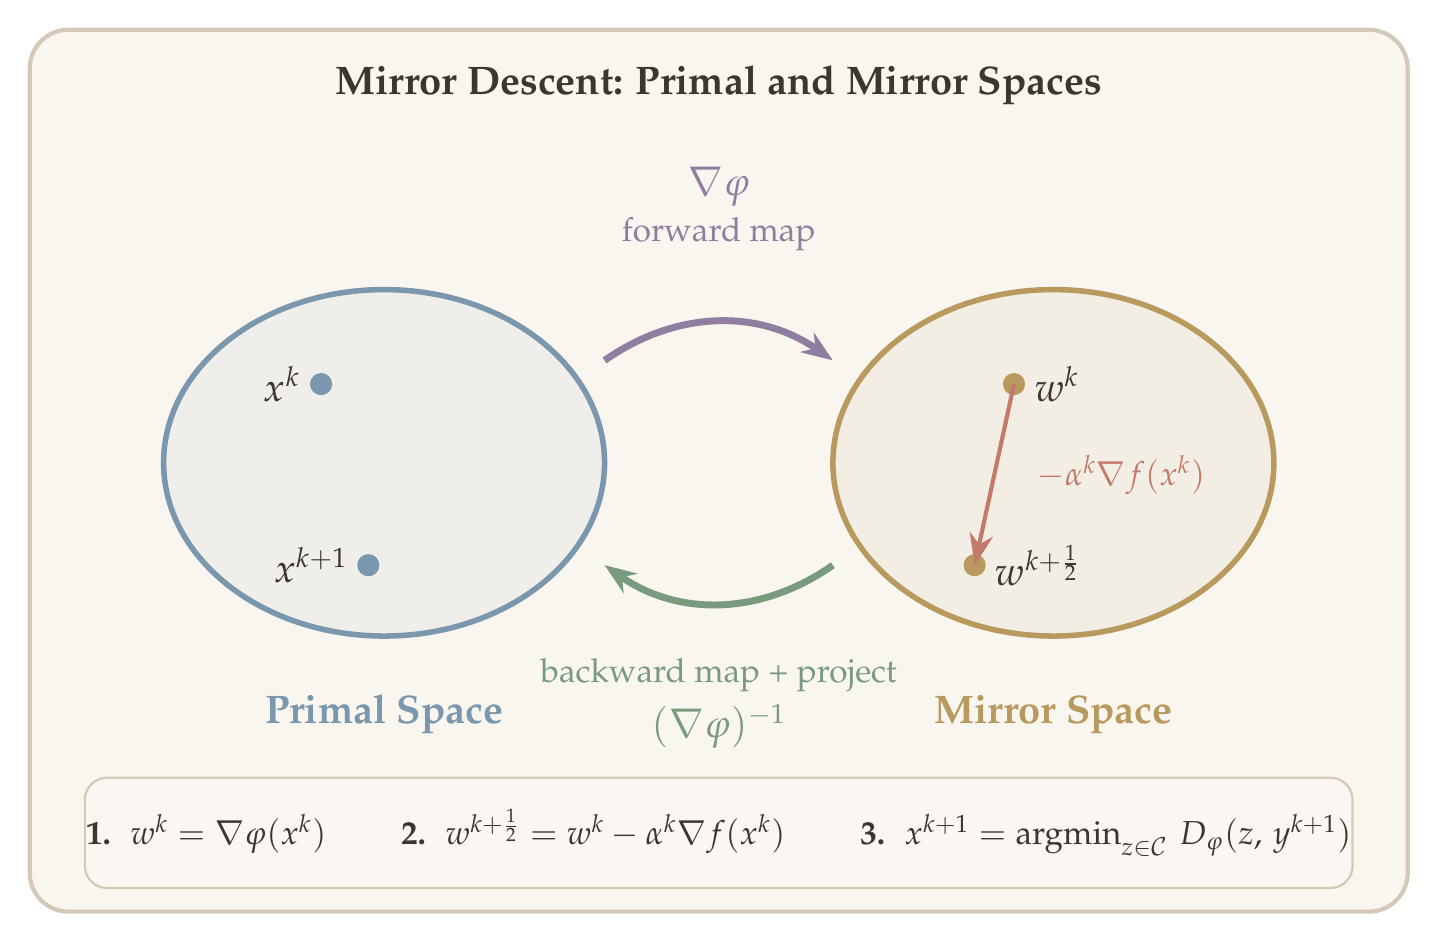
\begin{tikzpicture}[>={Stealth[length=4mm, width=3mm]}]

% Background
\fill[cream, rounded corners=14pt] (-0.5,-1.2) rectangle (17,10);
\draw[border, line width=1.5pt, rounded corners=14pt] (-0.5,-1.2) rectangle (17,10);

% Title
\node[text=dkbrown, font=\Large\bfseries] at (8.25,9.3)
  {Mirror Descent: Primal and Mirror Spaces};

% --- Primal Space (left) ---
\coordinate (Pcenter) at (4.0,4.5);
\fill[stblue, opacity=0.08] (Pcenter) ellipse (2.8 and 2.2);
\draw[stblue, line width=2pt] (Pcenter) ellipse (2.8 and 2.2);

% Label
\node[text=stblue, font=\Large\bfseries] at (4.0,1.3) {Primal Space};

% Points in primal
\coordinate (xk) at (3.2,5.5);
\coordinate (xk1) at (3.8,3.2);

\fill[stblue] (xk) circle (4pt);
\node[text=dkbrown, font=\Large, left=4pt] at (xk) {$x^k$};
\fill[stblue] (xk1) circle (4pt);
\node[text=dkbrown, font=\Large, left=4pt] at (xk1) {$x^{k+1}$};


% --- Mirror Space (right) ---
\coordinate (Mcenter) at (12.5,4.5);
\fill[rwgold, opacity=0.08] (Mcenter) ellipse (2.8 and 2.2);
\draw[rwgold, line width=2pt] (Mcenter) ellipse (2.8 and 2.2);

% Label
\node[text=rwgold, font=\Large\bfseries] at (12.5,1.3) {Mirror Space};

% Points in mirror space
\coordinate (wk) at (12.0,5.5);
\coordinate (wk05) at (11.5,3.2);

\fill[rwgold] (wk) circle (4pt);
\node[text=dkbrown, font=\Large, right=4pt] at (wk) {$w^k$};
\fill[rwgold] (wk05) circle (4pt);
\node[text=dkbrown, font=\Large, right=4pt] at (wk05) {$w^{k+\frac{1}{2}}$};

% Gradient step arrow in mirror space
\draw[terracotta, line width=1.5pt, ->] (wk) -- (wk05);
\node[text=terracotta, font=\large, right=12pt] at ($(wk)!0.5!(wk05)$) {$-\alpha^k \nabla f(x^k)$};

% --- Forward map: primal -> mirror (curved above) ---
\draw[lavender, line width=2.5pt, ->] (6.8,5.8) to[bend left=35] (9.7,5.8);
\node[text=lavender, font=\Large\bfseries] at (8.25,8.0) {$\nabla\varphi$};
\node[text=lavender, font=\large] at (8.25,7.4) {forward map};

% --- Backward map: mirror -> primal (curved below) ---
\draw[sage, line width=2.5pt, ->] (9.7,3.2) to[bend left=35] (6.8,3.2);
\node[text=sage, font=\Large\bfseries] at (8.25,1.15) {$(\nabla\varphi)^{-1}$};
\node[text=sage, font=\large] at (8.25,1.8) {backward map + project};

% --- Step descriptions ---
\fill[cream!90!white, rounded corners=8pt] (0.2,-0.9) rectangle (16.3,0.5);
\draw[border, line width=0.8pt, rounded corners=8pt] (0.2,-0.9) rectangle (16.3,0.5);
\node[text=dkbrown, font=\large, align=center] at (8.25,-0.2)
  {\textbf{1.}\; $w^k = \nabla\varphi(x^k)$ \qquad
   \textbf{2.}\; $w^{k+\frac{1}{2}} = w^k - \alpha^k \nabla f(x^k)$ \qquad
   \textbf{3.}\; $x^{k+1} = \operatorname*{argmin}_{z \in \mathcal{C}}\, D_\varphi(z,\, y^{k+1})$};

\end{tikzpicture}
\end{document}
